\documentclass[12pt]{article}
\usepackage{cite}
\usepackage{color}
\usepackage{graphicx}
\usepackage{caption}
\usepackage{subcaption}
\usepackage{parskip}

\setlength{\parskip}{5pt}
\setlength{\parindent}{0pt}

\title{LC/MS Chromatogram Smoothing With Generative Adversarial Networks}

\author{Gabriel Ferns(CS Senior) , Max Horowitz-Gelb(CS Senior)}

\begin{document}

\maketitle

\abstract{
Liquid Chromatography Mass Spectrometry is a powerful tool for identifying and quantifying proteins in a complex sample. High throughput methods of LC/MS such as DIA allow for analysis of samples with thousands of proteins. But this increase in throughput comes at the cost of a decrease in signal quality. This gives incentive for post extraction methods to clean and smooth chromatogram signal data. Here , using a new and powerful deep learning framework known as GANs \cite{GAN}, we attempt to smooth chromatograms, without distortion of the true underlying quantifiable data. 
\color{red}
Highlight results here
\color{black}
}

\section{Introduction}
DIA \cite{DIA} is a method of LC/MS for quanitifying thousands of proteins. In order to to do analyze thousands of proteins at the same time, DIA methods have one cycling through thousands of different m/z windows, where each window is used to quantify a single peptide. Because we are analyzing so many windows at each time, the dwell time, or time in which signal is extracted, must be very short. Because of this, the quality of the data extracted can be quite poor. An alternative to DIA is SRM, or Selected Reaction Monitoring,\cite{SRM}. SRM is not good for quantifying more than a handful of peptides at a time, but the data generated is of far superior quality to DIA. It would be nice if we could keep the high throughput of DIA while also having data with the same quality as SRM. Then one could analyze thousands of proteins at the same time and get clean reliable data for quantification.

The quality of SRM data in comparison to DIA data suggests that perhaps a generative model trained on clean SRM data, could remove noise and smooth DIA data without distorting the actual quantifiable information. To test this hypothesis we chose to use a GAN as our generative model. GAN neural networks have been shown as powerful tools for image processing particularly for removal of noise and upscaling of images \cite{SRGAN}\cite{DERAIN}. We applied similar methods to chromatogram data by training a GAN on clean SRM data with simulated Gaussian noise. We then tested our GAN on a dataset of real DIA data.

\color{red}
Include results here
\color{black}

\begin{figure}
\centering
\begin{subfigure}{.5\textwidth}
  \centering
  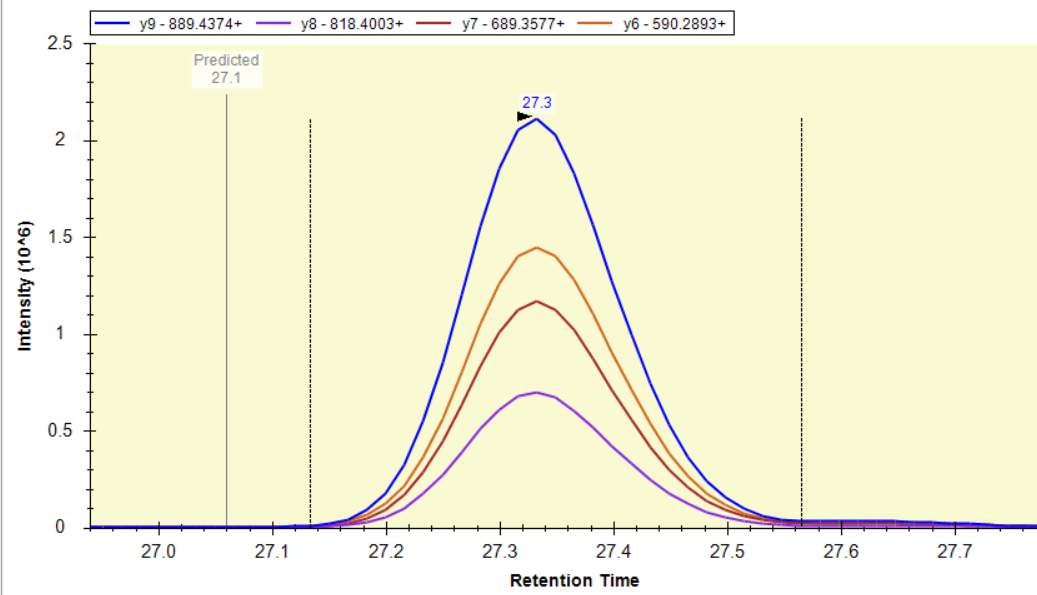
\includegraphics[width=1\linewidth]{smoothExample.png}
  \caption{SRM Chromatogram}
  \label{fig:sub1}
\end{subfigure}%
\begin{subfigure}{.5\textwidth}
  \centering
  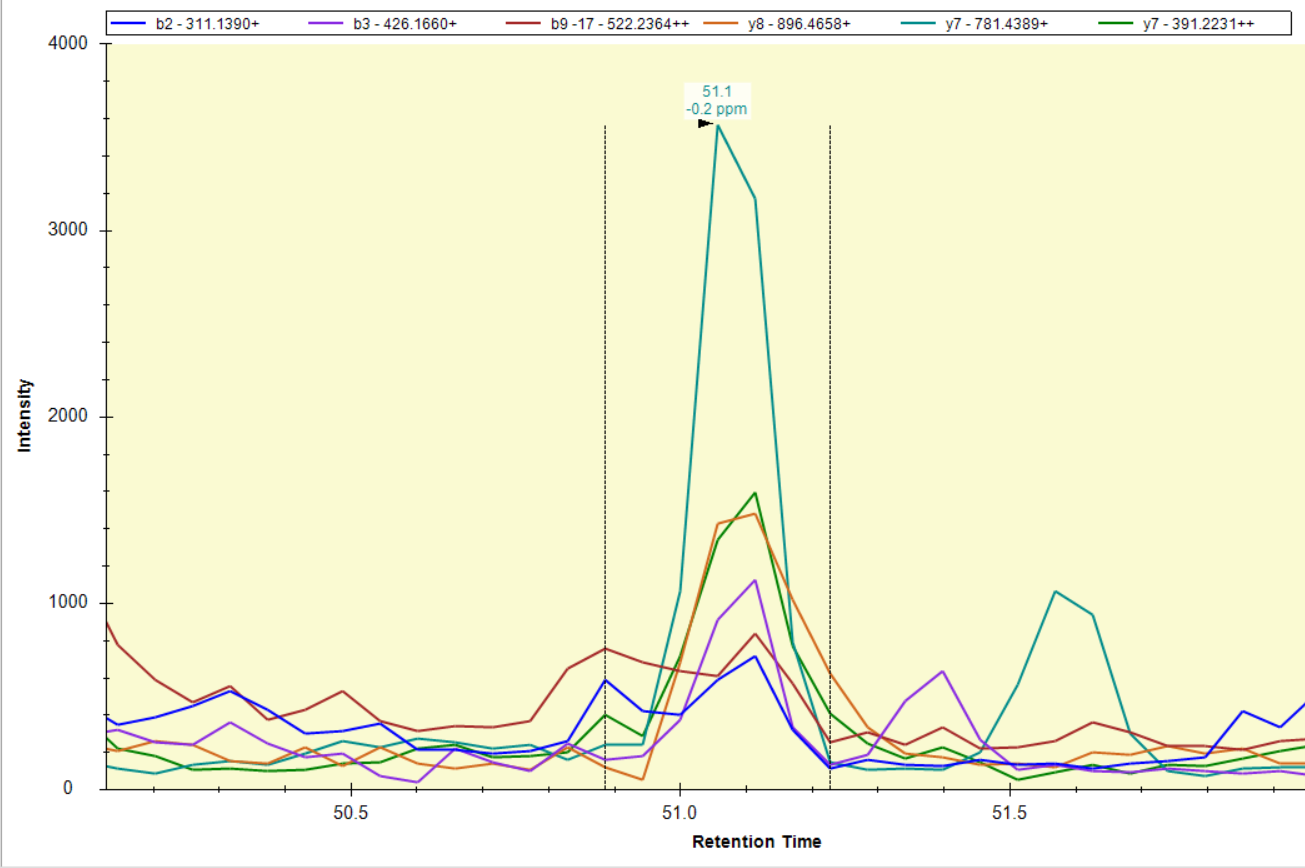
\includegraphics[width=1\linewidth]{DIA_example}
  \caption{DIA Chromatogram}
  \label{fig:sub2}
\end{subfigure}
\caption{Here we show two chromatograms. As one can see the noise and the smoothness is much better in the chromatogram coming from an SRM dataset.}
\label{fig:test}
\end{figure}

\section{Brief LC/MS Primer}
LC/MS identifies and quantifies proteins by separating them by their hydrophobicity and mass. In general it is difficult to quantify whole proteins so we instead use peptides which are sub-sequences of a protein. These peptides come off of a liquid column at a specific time which is dependent on the hydrophobicity of the peptide.This time is known as the peptide's Retention Time. Once the peptide comes off the column it is ionized and then becomes what is called a precursor ion. When precursor ions go into the mass spectrometer they are filtered by the ratio of their mass to charge. A precursor ion's mass to charge along with its retention time are used as a two fold filtration process for unique quantification of peptides. 

At this point one could start quantifying the peptide, but in certain methods, like DIA, the precursor is then blasted it with an ion spray. This ion spray causes the precursor to fragment into two pieces. One of these pieces, known as a transition ion, becomes charged and may be detected by the machine. The ratio of expected number of transition ions for each possible fragment that could occur is known via empirical evidence. Because of this the relative ion intensity of each transition ion is useful for identification of the peptide.

\begin{figure}
\centering
\begin{subfigure}{.5\textwidth}
  \centering
  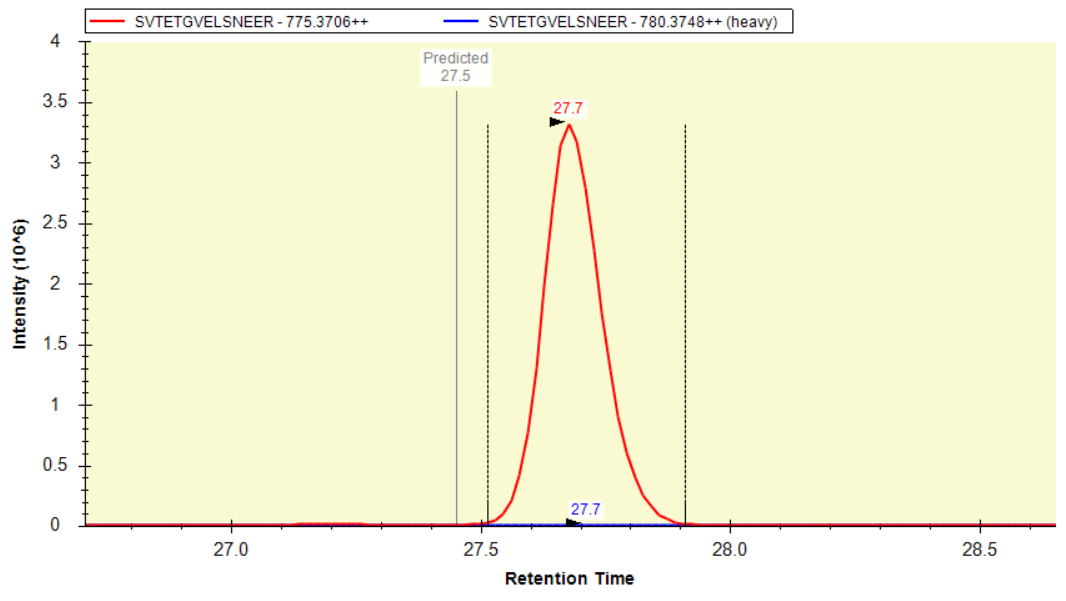
\includegraphics[width=1\linewidth]{precursor}
  \caption{Precursor Chromatogram}
  \label{fig:sub1}
\end{subfigure}%
\begin{subfigure}{.5\textwidth}
  \centering
  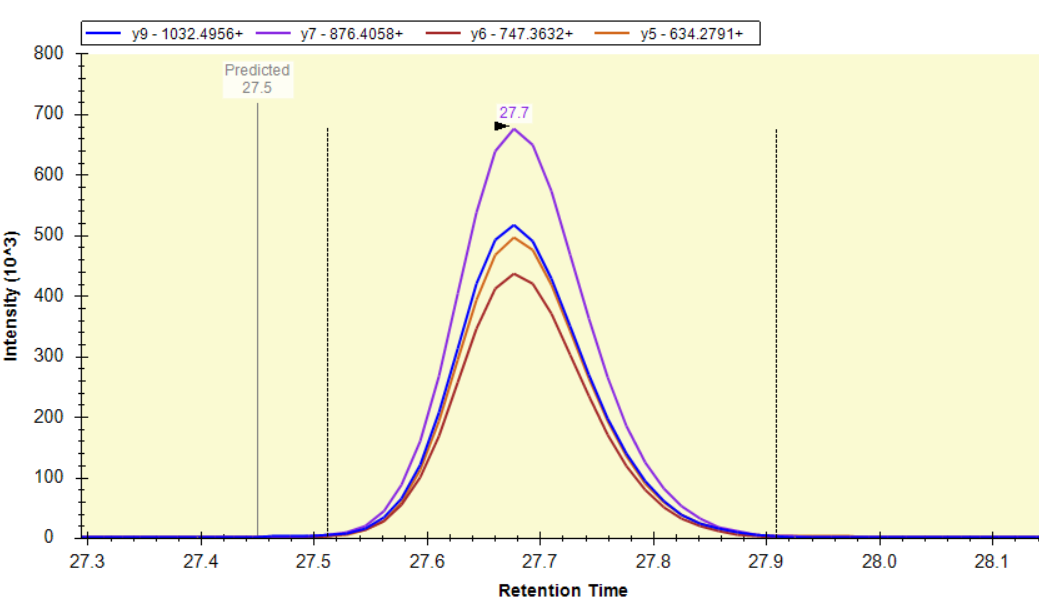
\includegraphics[width=1\linewidth]{transitions}
  \caption{Transition Chromatograms(Peak Group)}
  \label{fig:sub2}
\end{subfigure}
\caption{Here we show the difference between precursor and transition ion chromatograms. The precursor chromatogram contains a single peak, while the transition chromatogram shows a set of peaks coming from all the different transitions or fragment ions. This set of transition chromatograms coming from the same peptide is known as a peak group.}
\label{fig:test}
\end{figure}


\section{Task Definition}
The goal of this project is to train a GAN so that it can take a peak group and return the same peak group after being smoothed and denoised.  
The GAN smooths and denoises each transition separately. The network takes as input the chromatogram from a single transition as well as an average signal from all the other transitions coming from the same peak group.  The reason this is done is that as one can see from figure 2, each transition chromatogram has a similar shape to all the other chromatograms in the peak group. So having an average of the other chromatograms is a clue into the true shape of the transition chromatogram we are trying to smooth. 

The GAN takes the average chromatogram and the single transition chromatogram as input and then outputs a chromatogram of the single transition after it has been smoothed. 

\begin{figure}
\centering
\begin{subfigure}{.5\textwidth}
  \centering
  %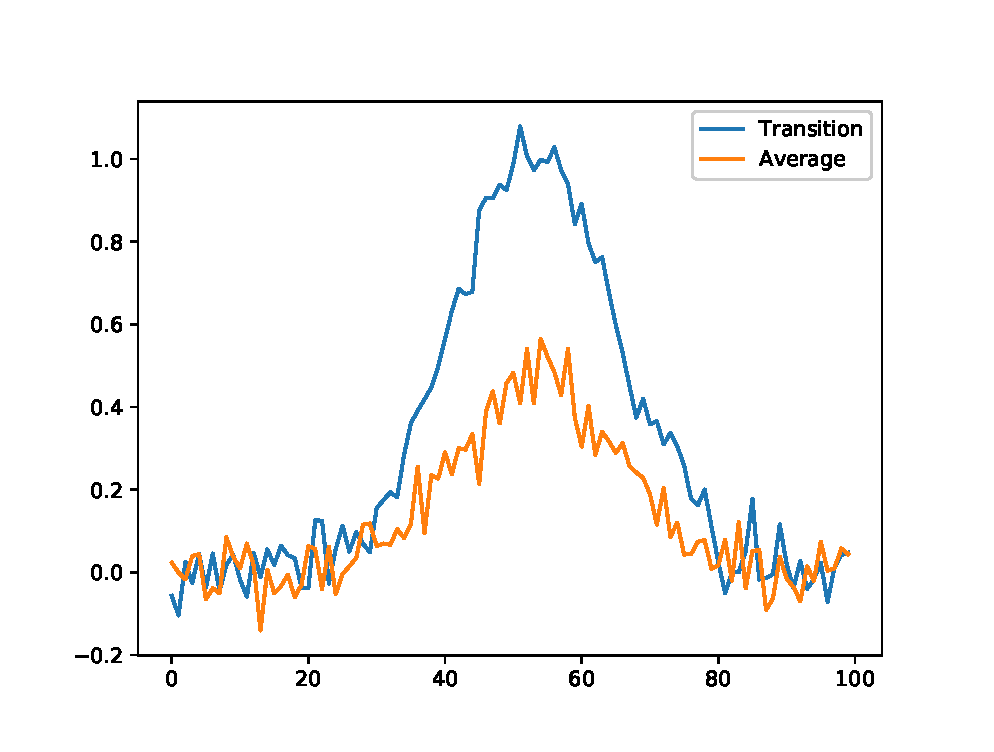
\includegraphics[width=1\linewidth]{input}
  \caption{Input}
  \label{fig:sub1}
\end{subfigure}%
\begin{subfigure}{.5\textwidth}
  \centering
  %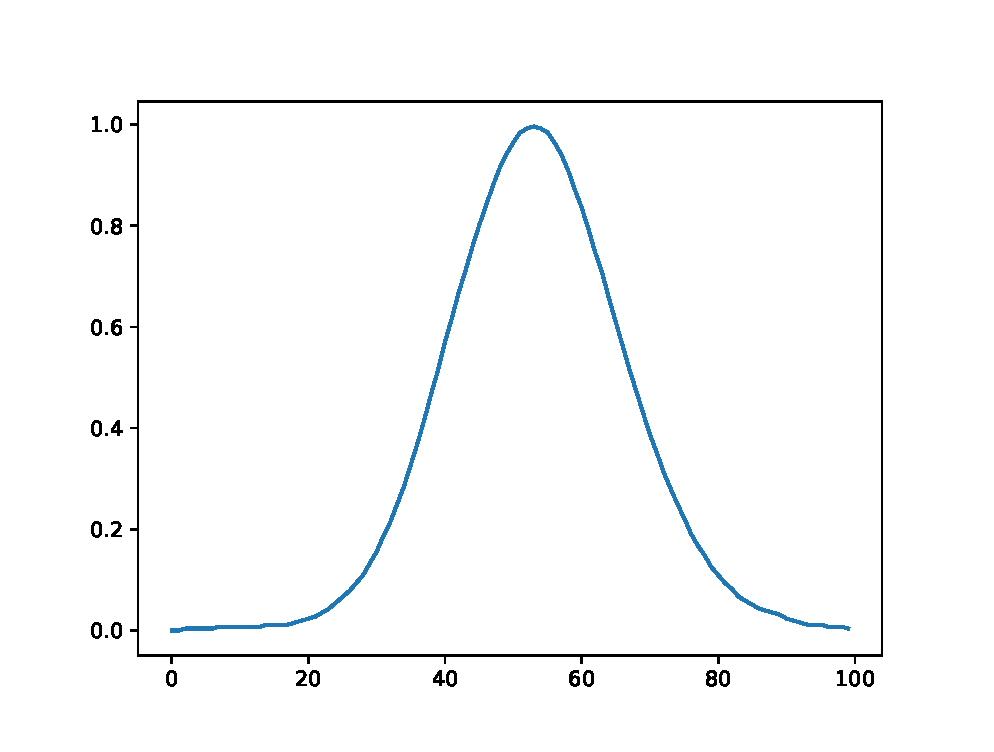
\includegraphics[width=1\linewidth]{output}
  \caption{Output}
  \label{fig:sub2}
\end{subfigure}
\caption{Here we show the input and output data for the GAN network. The input composes of unique transition along with an average shape chromatogram coming from all other transitions in the peak group. The output is the smoothed peak group from the transition. (Note the above is not real input or output data as a result of training. It is only for demonstration)}
\label{fig:test}
\end{figure}

\color{red}
Gabe describe structure of the Gans net. 
\color{black}
\section{Algorithm Definition}
\subsection{Chromatogram Pre-processing}
Before we can use the chromatogram data it has to be pre-processed. The time span of each peakgroup is not of equal length so all the chromatograms had to be up-sampled or down-sampled so that they were all a standard length of 100 intensity points per peak. As well the intensities were normalized to range from 0 to 1.   
\subsection{GAN}
\color{red}
Gabe explain GANs.
\color{black}
\section{Methodology}
For training we used a high qualitiy SRM dataset\cite{smooth_Data} containing approximately 12,000 unique transition chromatograms. For our testing, we used DIA dataset \cite{TRIC} of 16 samples each containing 500 peakgroups.

For the test data, we only had the noisy raw DIA data. We don't know what the true shape of the peaks should look like once the noise was removed. For a single peak group the only way to know if we correctly smoothed the data without distorting it would be if we knew beforehand the true amount of protein that existed in each sample. Unfortunately we did not know that for the sample we were using. 

So instead we used relative ion intensity to measure the quality of our data. As mentioned earlier in the primer, the relative intensity of each fragment ion has a fairly stable value which we can use for identification. In the test set we have 16 different samples all containing the same peptides. If after smoothing the test data we found that the relative ion intensties for the same peptide across samples didn't match, then we would know that we had corrupted the data. 

To calculate this metric we simply integrate over the curve of each ion's chromatogram in the same peak group. Combing these integrations gives a vector of chromatogram areas for each peptide in each sample. Then with these vectors we simply calculate the average cosine angle between all different samples for the same peptide. This average is our score, where 1 is the best and -1 is the worst.

If after doing smoothing from GANS we see this score go significantly down from before smoothing, then we know that we are corrupting the data. But if it is close to 1, then we can feel confident that the GAN is smoothing the data correctly. 
\section{Results}
\section{Discussion}
\section{Individual Contributions}

\section{Related Work}
\section{Future Work}
\section{Conclusion}

\bibliography{writeup}{}
\bibliographystyle{plain}

\end{document}